%%%%%%%%%%%%%%%%%%%%%%%%%%%%%%%%%%%%%%%%%%%%%%%%%%%%%%%%%%%%%%%%%%%%%%%%%%%%%%%%%%%%
% Document data
%%%%%%%%%%%%%%%%%%%%%%%%%%%%%%%%%%%%%%%%%%%%%%%%%%%%%%%%%%%%%%%%%%%%%%%%%%%%%%%%%%%%
\documentclass[12pt]{article} %report allows for chapters
%%%%%%%%%%%%%%%%%%%%%%%%%%%%%%%%%%%%%%%%%%%%%%%%%%%%%%%%%%%%%%%%%%%%%%%%%%%%%%%%%%%%
\usepackage{preamble}

\begin{document}

\begin{center}
   \textsc{\large MATH 271, Homework 0, \emph{Solutions}}\\
   \textsc{Due August 30$^\textrm{th}$}
\end{center}

\begin{center}
    \textbf{Tell me a little bit about yourself!}
\end{center}

\begin{question}
    Where did you grow up? Why did you choose Colorado State University?
\end{question}

\begin{answer}
    I grew up in Pasadena which is in southern California.  I chose to come to CSU as an undergraduate student since I loved the area when I came to visit.  The mountains are really great, and I don't miss the beaches.  Also, I was very interested in veterinary science and this was a great school for that! I've been here ever since.
\end{answer}

\hrule

\begin{question}
    What is something interesting about yourself.  What is a favorite hobby of yours?
\end{question}

\begin{answer}
    I went to Italy for two weeks and ate pizza every single day I was there. My favorite hobby is mountain biking. I ride anything. Cross country, downhill, dirt jumps, doesn't matter!  I'm trying to get into climbing and hiking more as well.
\end{answer}

\hrule

\begin{question}
    Why are you interested in chemistry? Do you have plans after you earn your degree?
\end{question}

\begin{answer}
    Well, I'm interested in chemistry because it is the study of interactions at a level that we all, well, interact with.  Physics can study phenomena on scales that are too large or too small for humans to really comprehend but chemistry sits at just the right vantage point.  I'm not sure what I'll do after I earn my Ph.D. We'll see where it takes me I suppose!
\end{answer}

\hrule

\begin{question}
    Honest answers appreciated here.  Do you enjoy mathematics? Do you think it's hard? What do you hope to gain from this course?
\end{question}

\begin{answer}
    Yes, I do.  I didn't use to though.  I thought it was a bit tedious and pointless.  However, I never really thought it was too hard. Once I got into more advanced mathematics courses, I thought it was more difficult than physics or engineering. That's part of what drove me to pursue it! 
    
    One should not worry if mathematics feels hard to them.  For me, plenty of other things are difficult and take me much more work to conceptualize. Everyone has their skills and everyone has to work to improve.  There's a stigma associated with mathematics in this country, and I will do my best to dispell this belief. 
    
    I hope to learn more chemistry from this course than I currently know. Also, I'd like to grow as a teacher.  I thoroughly enjoy teaching. It makes me happy to share some knowledge with my students!
    
\end{answer}

\hrule

\begin{center}
    \textbf{Now for some mathematics.}
\end{center}

\begin{problem}
    Compute the following:
\begin{enumerate}[(a)]
    \item $\displaystyle{\frac{d}{dx}(2x^7-3x^4+7)}$;
    \item $\displaystyle{\frac{d}{dt}\left(e^{at}\sin(bt)\right)}$;
    \item $\displaystyle{\frac{d}{ds}\left(\tan\left( e^{s^2}\right)\right)}$.
\end{enumerate}
\end{problem}

\begin{solution}~
\begin{enumerate}[(a)]
    \item Using the power, sum, and constant multiple rules we get
    \[
    \frac{d}{dx}\left( 2x^7 -3x^4 +y\right) = 14x^6-12x^3.
    \]
    \item Now using product and chain rule, we have
    \[
    \frac{d}{dt}\left( e^{at}\sin(bt)\right)= ae^{at}\sin(bt)+be^{at}\cos(bt).
    \]
    \item Using the chain rule twice, we have
    \[
    \frac{d}{ds} \left( \tan\left( e^{s^2}\right)\right) = \sec^2\left(e^{s^2}\right)2se^{s^2}.
    \]
\end{enumerate}
\end{solution}

\hrule

\begin{problem}
    Compute the following:
\begin{enumerate}[(a)]
    \item $\displaystyle{\int 2x^7-3x^4+7dx}$;
    \item $\displaystyle{\int_{-1}^1 \cos(t) dt}$;
    \item $\displaystyle{\int_0^1 e^{2y}dy}$;
\end{enumerate}
\end{problem}

\begin{solution}
~
\begin{enumerate}[(a)]
    \item Here, we use the power rule for antiderivatives to get
    \[
    \frac{1}{4} x^8 - \frac{3}{5} x^5 + 7x + c,
    \]
    where $c$ is an undetermined constant.
    \item Cosine is an \emph{even} function meaning that
    \[
    \cos(x)=\cos(-x).
    \]
    So we have
    \[
    \int_{-1}^1 \cos(t) dt = 2\int_0^1 \cos(t)dt.
    \]
    Then we use the fundamental theorem of calculus to get
    \[
    2\int_0^1 \cos(t)dt = 2 ( \sin(1)-\sin(0))=2\sin(1).
    \]
    \item Here, we need to make a substitution in that $z=2y$ so $dz=2dy$. Then we get
    \[
    \int_0^1 e^{2y}dy = \frac{1}{2} \int_0^2e^{z}dz.
    \]
    Then we can evaluate
    \[
    \frac{1}{2}\int_0^2 e^z dz = \frac{1}{2}\left(e^2-1\right).
    \]
\end{enumerate}
\end{solution}

\hrule

\begin{problem}
    Find the point(s) of intersection of the parabola $f(x)=2x^2+2x+2$ and the line $g(x)=4x+4$. Draw a picture and identify what's happening. (You can plot this on Desmos and print that out if you'd like, but do the algebra to find the solution by hand.)
\end{problem}

\begin{solution}
Here's a picture of the two curves.
\begin{figure}[H]
    \centering
    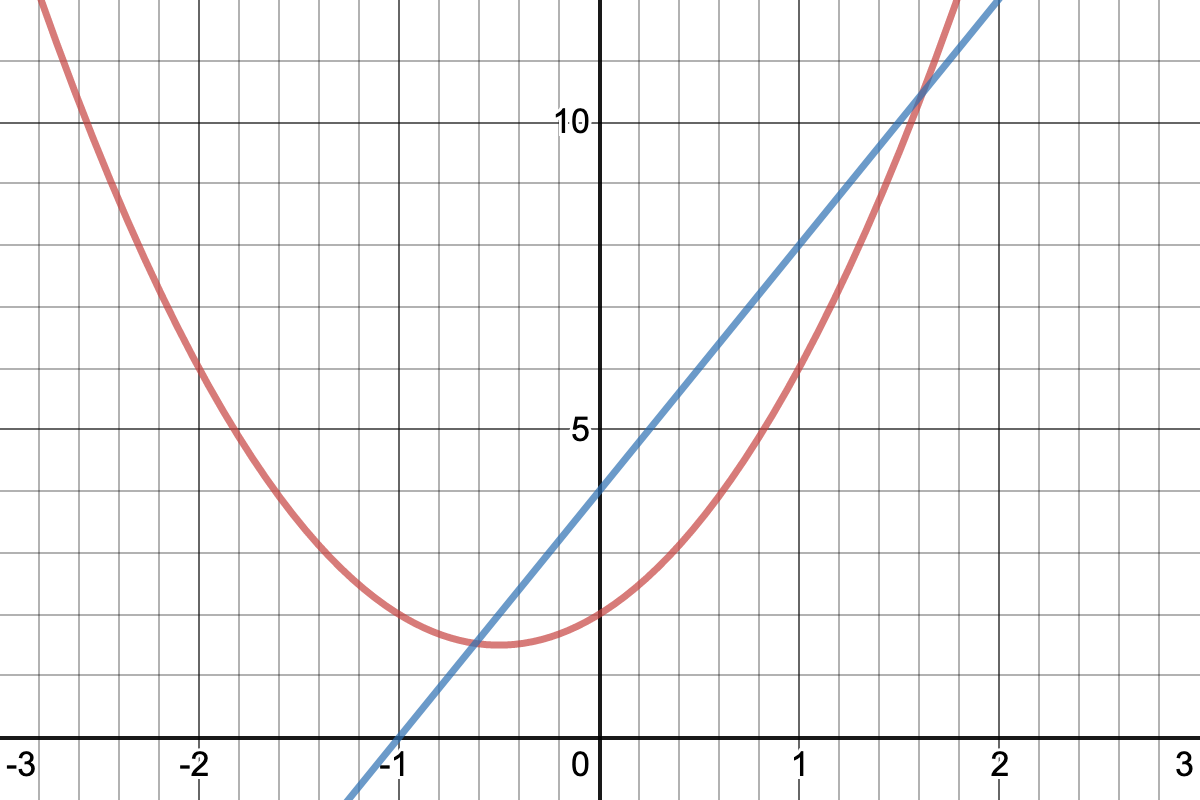
\includegraphics[width=.8\textwidth]{desmos-graph.png}
\end{figure}
We can see that they interesect in two points. We can find these intersections by setting the functions equal
\[
f(x)=g(x)
\]
which gives us
\begin{align*}
    2x^2+2x+2&=4x+4\\
    2x^2-2x-2&=0.
\end{align*}
So we can find the intersections by finding roots to a different (associated) polynomial. The roots (and thus intersections) are
\[
x=\frac{1}{2}\pm \frac{\sqrt{5}}{2}.
\]
\end{solution}

\hrule

\begin{problem}
    Now take the same parabola $f(x)=2x^2+2x+2$ and the line $h(x)=4x-4$. Draw a picture to show that these parabolas do not intersect. We can find ``complex intersections" by doing the same algebra as the previous problem. Find these complex interesctions. (\emph{Hint: set up an equation whose roots would give you the intersections of these two curves.)}
\end{problem}

\hrule

\begin{solution}
Here's another picture.
\begin{figure}[H]
    \centering
    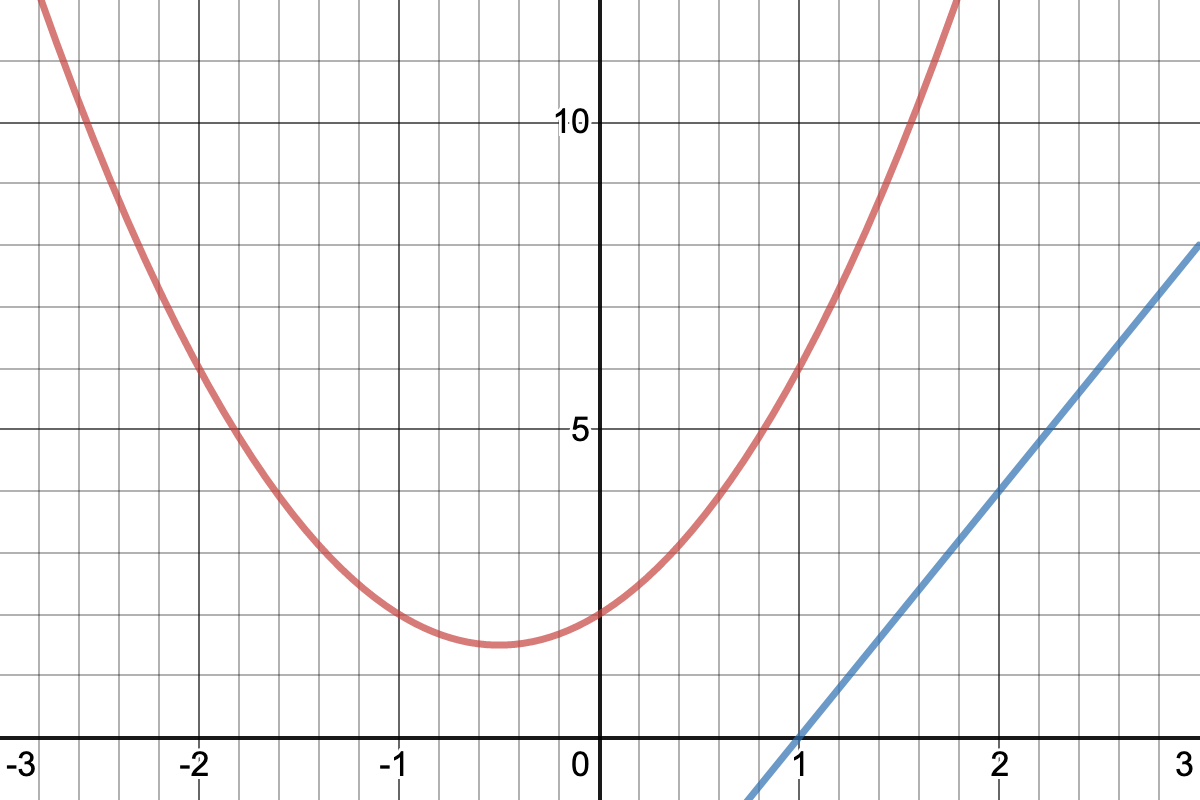
\includegraphics[width=.8\textwidth]{desmos-graph(2).png}
\end{figure}
Notice that these curves do not intersect when we allow only real number inputs. However, if we allow for complex inputs, then the functions can be equal. Algebraically, we have
\begin{align*}
    f(x)&=h(x)\\
    2x^2+2x+2&= 4x-4\\
    2x^2-2x+6&=0.
\end{align*}
The roots (or interesections) for this polynomial are then
\[
x=\frac{1}{2}\left( 1 \pm i \sqrt{11}\right).
\]
If you get used to complex numbers, you can wear your complex-goggles and see the interesection here! Honestly, I'm not great at wearing complex-goggles.
\end{solution}

\end{document}